% $Id$
%==============================================================================
\section{Summary}
\label{section:LoginExampleSummary}
%==============================================================================

In this chapter, a lot of different CCM Tools use cases have been shown.
Each use case satisfies a particular architectural requirement, but
the main advantage of CCM Tools comes from a combination of these use cases. 

\begin{figure}[htbp]
    \begin{center}
        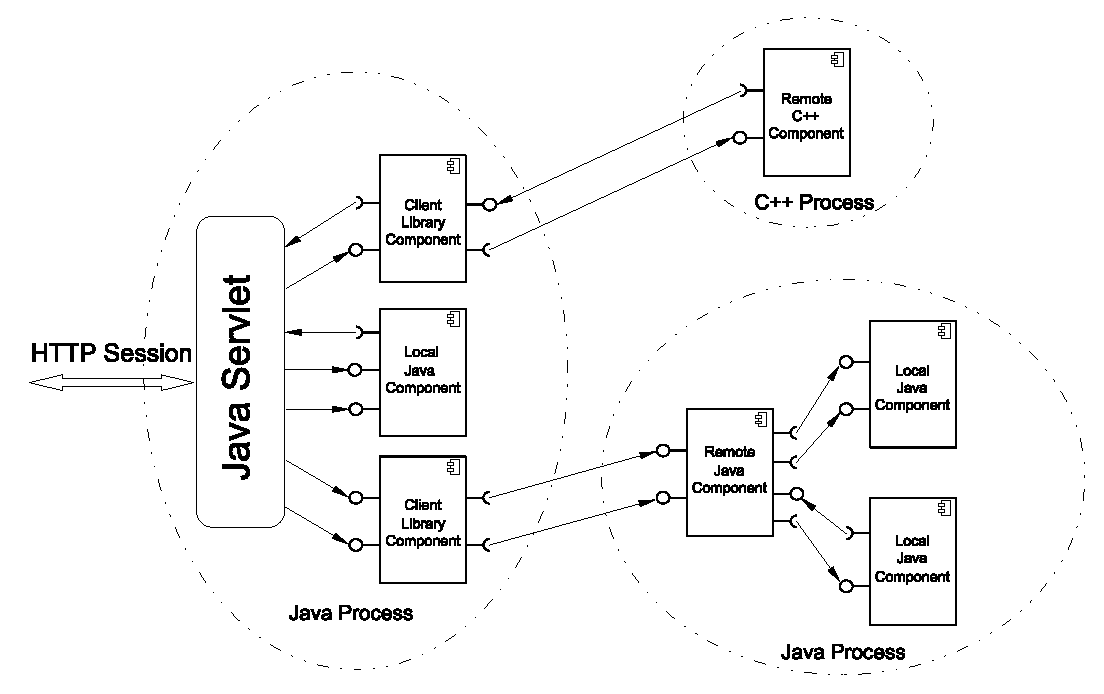
\includegraphics [width=14cm,angle=0] {figures/LoginSummary}
        \caption{Combining different CCM Tools use cases.}
        \label{figure:LoginSummery}
    \end{center}
\end{figure}

Fig.~\ref{figure:LoginSummery} shows a possible scenario where different use
cases are combined to realize a 	heterogeneous and distributed software system.
Based on CORBA middleware, we can interact between C++ and Java remote
components as well as between remote components and Java client library
components.

\vspace{3mm}
As component developers, we defined components in IDL and implement business
logic in generated implementation skeleton classes. 
Structural code needed to establish components which can be instantiated and 
connected via facts and receptacles, either local or remote, is completely generated by the
CCM Tools.






\newpage


